
\chapter{해석적 방법 (Analytic methods)}
\label{analysis}

이책은 모의시험이나 재표본추출같은 수치해석적 방법(computational methods)에 집중했지만, 해결한 문제중 일부는 훨씬더 빠르게 해결할 수 있는 해석적 해(analytic solution)를 가지고 있다.
\index{재표본추출 (resampling)}
\index{해석적 방법 (analytic methods)}
\index{수치해석적 방법 (computational methods)}

이번 장에서 해석적 방법 일부를 제시하고, 어떻게 동작하는지 설명한다. 이장말미에 탐색적 데이터 분석을 위해서 수치해석적 방법과 해석적 방법 통합에 대한 제언을 한다.

이번 장에서 사용되는 코드는 {\tt normal.py}에 있다.
코드를 다운로드하고 작업하는 것에 대한 정보는 ~\ref{code}을 참조한다.


\section{정규분포}
\label{why_normal}
\index{정규분포 (normal distribution)}
\index{분포(distribution)!정규(normal)}
\index{가우스 분포 (Gaussian distribution)}
\index{분포 (distribution)!가우스 (Gaussian)}

동기부여를 위한 사례로, ~\ref{gorilla} 절에 있던 문제를 검토하자.
\index{고릴라 (gorilla)}

\begin{quotation}
\noindent 야생동물 보호구에서 고릴라를 연구하는 과학자가 있다고 가정하자. 고릴라 9마리 체중을 재서, 표본평균 $\xbar=90$ kg와 표본 표준편차 $S=7.5$ kg을 얻었다. 만약 $\xbar$를 모집단 평균으로 추정한다면, 추정값의 표준오차는 얼마나 될까?
\end{quotation}

이 질문에 대답하기 위해서, $\xbar$ 표집 분포가 필요하다. ~\ref{gorilla}절에서, (고릴라 9마리 체중을 재는) 실험을 모의시험함으로써 분포를 근사했고, 각 모의시험 실험에 대해서 $\xbar$를 계산하고, 추정값 분포를 축적했다.
\index{표준오차 (standard error)}
\index{표준편차 (standard deviation)}

결과는 표집분포를 근사했다. 그리고 나서, 표집분포를 사용해서 표준오차와 신뢰구간을 계산했다.
\index{신뢰구간 (confidence interval)}
\index{표집분포 (sampling distribution)}

\begin{enumerate}

\item 표집분포 표준편차는 추정값의 표준오차다; 이 경우 약 2.5 kg이 된다.

\item 5번째와 95번째 백분위수 표집분포 구간이 90\% 신뢰구간이 된다. 만약 실험을 많이 수행한다면, 추정값이 90\% 신뢰구간에 떨어질 것으로 예상한다. 이 경우 90\% CI는 $(86, 94)$ kg이 된다.

\end{enumerate}

이제 해석적으로 동일한 계산을 수행한다. 성인 여성 고릴라 체중이 대략 정규분포한다는 사실을 이용한다.
정규분포는 분석을 용이하게 하는 성질을 두개 갖고 있다; 선형 변환과 덧셈에 ``닫혀(closed)''있다.
이것이 의미하는 바를 설명하기 위해서, 약간의 표기가 필요하다. 
\index{분석 (analysis)}
\index{선형변환 (linear transformation)}
\index{덧셈, 닫혀있다. (addition, closed under)}

어떤 양(quantity)의 분포 $X$가 모수 $\mu$와 $\sigma$을 갖는 정규분포라면, 다음과 같이 표현할 수 있다.
%
\[ X \sim \normal~(\mu, \sigma^{2})\]
%
여기서, 기호 $\sim$ 는 ``분포한다(is distributed)''를 의미하고, 스크립트 문자 $\normal$는 ``정규(normal)''를 나타낸다.

%The other analytic distributions in this chapter are sometimes
%written $\mathrm{Exponential}(\lambda)$, $\mathrm{Pareto}(x_m,
%\alpha)$ and, for lognormal, $\mathrm{Log}-\normal~(\mu,
%\sigma^2)$.
$X$의 선형변환은 $X' = a X + b$와 같은 것으로, 여기서 $a$와 $b$는 실수다.
\index{선형변환 (linear transformation)}
만약, $X'$이 $X$와 같은 모임(족, family)이면, 분포 모임이 선형변환에 닫혀있다. 정규분포는 이 성질을 갖고 있다; 만약 $X \sim \normal~(\mu,
\sigma^2)$이면,
%
\[ X' \sim \normal~(a \mu + b, a^{2} \sigma^2) \tag*{(1)} \]
%
정규분포는 또한 덧셈에도 닫혀있다.
만약 $Z = X + Y$ 이고, $X \sim \normal~(\mu_{X}, \sigma_{X}^{2})$, $Y \sim \normal~(\mu_{Y}, \sigma_{Y}^{2})$이면,
%
\[ Z \sim \normal~(\mu_X + \mu_Y, \sigma_X^2 + \sigma_Y^2)  \tag*{(2)}\]
%
특별한 경우 $Z = X + X$이면, 다음을 만족한다.
%
\[ Z \sim \normal~(2 \mu_X, 2 \sigma_X^2) \]
%
그리고, 일반적으로 $X$에서 $n$개 값을 추출한다면, 다음을 갖게 된다.
%
\[ Z \sim \normal~(n \mu_X, n \sigma_X^2)  \tag*{(3)}\]


\section{표집분포}

이제 $\xbar$ 표집분포를 계산하는데 필요한 모든 것을 갖췄다. $\xbar$를 계산하는데 $n$개 고릴라 체중을 재고, 더해서 전체 체중값을 얻고 나서, $n$으로 나눈다는 것을 기억하라.
\index{표집분포 (sampling distribution)}
\index{고릴라 (gorilla)}
\index{체중 (weight)}

고릴라 체중 $X$ 분포가 근사적으로 정규분포라고 가정한다.
%
\[ X \sim \normal~(\mu, \sigma^2)\]
%
만약 $n$개 고릴라 체중을 잰다면, 전체체중 $Y$는 3번 방정식을 사용해서 다음과 같이 분포한다.
%
\[ Y \sim \normal~(n \mu, n \sigma^2) \]
%

그리고 만약 $n$으로 나눈다면, $a = 1/n$으로 1번 방정식을 사용해서 표본평균 $Z$는 다음과 같이 분포한다.
%
\[ Z \sim \normal~(\mu, \sigma^2/n) \]
%

$Z$ 분포는 $\xbar$의 표집분포가 된다.
$Z$ 평균은 $\mu$으로, $\xbar$가 $\mu$의 불편 추정값이 된다는 것을 보여준다.
표집분포 분산은 $\sigma^2 / n$이다.
\index{편의 추정량 (biased estimator)}
\index{추정량 (estimator)!편의 (biased)}

그래서, 표집분포 표준편차, 즉 추정값의 표준오차는 $\sigma / \sqrt{n}$이 된다. 예제에서, $\sigma$는 7.5 kg 이고, $n$은 9가 되서, 표준오차는 2.5 kg가 된다.
결과는 모의시험으로 추정한 것과 일치하지만, 계산하기는 훨씬 더 빠르다!
\index{표준오차 (standard error)}
\index{표준편차 (standard deviation)}

또한, 표집분포를 사용해서 신뢰구간도 계산할 수 있다.
$\xbar$에 대한 90\% 신뢰구간은 $Z$의 5번째와 95번째 백분위수 간격이다.
$Z$이 정규분포를 따르기 때문에, 역 CDF(inverse CDF)를 평가해서 백분위수를 계산할 수 있다.
\index{역 CDF (inverse CDF)}
\index{CDF, 역 (CDF, inverse)}
\index{신뢰구간 (confidence interval)}

정규분포 CDF와 역 CDF에 대한 닫힌 형태(closed form)가 존재하지 않지만, 
빠른 수치해석 방법이 존재하고 ~\ref{normal}절에서 살펴본 바와 같이 SciPy에 
구현되어 있다. {\tt thinkstats2}에 SciPy 함수를 좀더 쉽게 사용할 수 있게 하는 랩퍼(wrapper) 함수가 제공된다.
\index{SciPy}
\index{정규분포 (normal distribution)}
\index{랩퍼 (wrapper)}
\index{닫힌 형태 (closed form)}

\begin{verbatim}
def EvalNormalCdfInverse(p, mu=0, sigma=1):
    return scipy.stats.norm.ppf(p, loc=mu, scale=sigma)
\end{verbatim}

확률 {\tt p}가 주어졌을 대, 모수 {\tt mu}와 {\tt sigma}를 갖는 정규분포에서 대응되는 백분위수를 반환한다. 
$\xbar$의 90\% 신뢰구간에 대해서, 
다음과 같이 5번째와 95번째 백분위수를 계산한다.
\index{백분위수 (percentile)}

\begin{verbatim}
>>> thinkstats2.EvalNormalCdfInverse(0.05, mu=90, sigma=2.5)
85.888

>>> thinkstats2.EvalNormalCdfInverse(0.95, mu=90, sigma=2.5)
94.112
\end{verbatim}

그래서, 만약 실험을 많이 반복한다면, 추정값 $\xbar$가 약 90\%로 범위 $(85.9, 94.1)$에 떨어질 것이다. 
다시 이값은 모의시험으로 얻은 결과와 일치한다.
\index{simulation}


\section{정규분포 표현하기}

상기 계산을 좀더 쉽게하기 위해서, {\tt Normal} 클래스를 정의하는데 정규분포를 표현하고 앞절 방정식을 부호화한다. 다음에 코드가 있다.
\index{Normal}

\begin{verbatim}
class Normal(object):

    def __init__(self, mu, sigma2):
        self.mu = mu
        self.sigma2 = sigma2

    def __str__(self):
        return 'N(%g, %g)' % (self.mu, self.sigma2)
\end{verbatim}

그래서, 고릴라 체중 분포를 표현하는 Normal을 인스턴스화할 수 있다.
\index{고릴라 (gorilla)}

\begin{verbatim}
>>> dist = Normal(90, 7.5**2)
>>> dist
N(90, 56.25)
\end{verbatim}

{\tt Normal} 클래스에는 {\tt Sum} 메쏘드가 제공되는데, 표본크기 {\tt n}을 인다로 받아, 방정식 3을 사용해서 {\tt n}개 값의 합계 분포를 반환한다.

\begin{verbatim}
    def Sum(self, n):
        return Normal(n * self.mu, n * self.sigma2)
\end{verbatim}

Normal은 또한 방정식 1을 사용해서 곱셈과 나눗셈도 수행한다.

\begin{verbatim}
    def __mul__(self, factor):
        return Normal(factor * self.mu, factor**2 * self.sigma2)

    def __div__(self, divisor):
        return 1 / divisor * self
\end{verbatim}

그래서, 표본크기 9를 가지고 평균의 표집분포를 계산할 수 있다.
\index{표집분포 (sampling distribution)}
\index{표본크기 (sample size)}

\begin{verbatim}
>>> dist_xbar = dist.Sum(9) / 9
>>> dist_xbar.sigma
2.5
\end{verbatim}

으로 앞절에서 살펴보았듯이, 표집분포 표준편차는 2.5 kg이다.
마지막으로, Normal 클래스에는 {\tt Percentile} 메쏘드가 있어서 신뢰구간을 계산하는데 사용할 수 있다.
\index{표준편차 (standard deviation)}
\index{신뢰구간 (confidence interval)}

\begin{verbatim}
>>> dist_xbar.Percentile(5), dist_xbar.Percentile(95)
85.888 94.113
\end{verbatim}

그리고, 이것은 앞에서 얻은 답과 같다. 나중에 Normal 클래스를 다시 사용할 것이다. 하지만, 더 진도를 나가기 전에, 분석 한가지가 더 필요하다.


\section{중심극한정리 (Central limit theorem)}
\label{CLT}

앞절에서 살펴봤듯이, 만약 정규분포에서 추출한 값을 더하면, 합 분포도 정규분포다. 다른 대부분의 분포는 이런 성질을 갖지 못하다; 만약 다른 분포에서 추출한 값을 더한다면, 합은 일반적으로 해석적 분포를 갖지 못한다.
\index{합(sum)}
\index{정규분포 (normal distribution)} \index{분포 (distribution)!정규 (normal)}
\index{가우스 분포 (Gaussian distribution)} \index{분포 (distribution)!가우스 (Gaussian)}

하지만, 거의 모든 분포에서 {\tt n} 값을 더하면, 합 분포가 {\tt n}이 증가함에 따라 정규분포로 수렴한다.

좀더 구체적으로, 만약 값들의 분포가 평균과 표준편차 $\mu$와 $\sigma$를 갖는다면, 합 분포는 근사적으로 $\normal(n \mu, n \sigma^2)$이 된다.
\index{표준편차 (standard deviation)}

이 결과가 중심극한정리(Central Limit Theorem, CLT)이다.  
통계분석을 위한 가장 유용한 도구 중 하나다. 하지만, 몇가지 주의점이 있다.
\index{중심극한정리 (Central Limit Theorem)}
\index{CLT}

\begin{itemize}

\item 값들이 독립적으로 추출되어야 한다. 만약 상관된다면, CLT을 적용할 수 없다.(설사 이것이 실무에서 문제가 결코되지는 않을지만)
\index{독립적 (independent)}

\item 값들이 동일한 분포에서 나와야 한다 (설사 이런 요구사항은 완화될 수도 있지만)
\index{동일한 (identical)}

\item 유한 평균과 분산을 갖는 분포에서 값들이 나와야 한다. 그래서 대부분 파레토 분포는 해당되지 않는다.
\index{평균 (mean)}
\index{분산 (variance)}
\index{파레토 분포 (Pareto distribution)}
\index{분포 (distribution)!파레토 (Pareto)}
\index{지수분포 (exponential distribution)}
\index{분포 (distribution)!지수 (exponential)}

\item 수렴 속도는 분포 왜도에 의존한다. 지수분포에서 나온 값들의 합은 작은 {\tt n}에 대해서 수렴한다. 로그 정규분포에서 나온 값들의 합은 더 커다란 크기가 필요하다.
\index{로그정규분포 (lognormal distribution)}
\index{분포 (distribution)!로그정규 (lognormal)}
\index{왜도 (skewness)}

\end{itemize}

중심극한정리는 자연 세계에 정규분포가 널리 퍼짐을 설명한다.
생물체의 많은 특징이 유전적 환경적 요인에 영향을 받는데, 이들 효과는 가법(additive)적이다. 측정하는 특징은 많은 작은 효과의 합이다. 그래서, 분포가 정규분포화 되는 경향이 있다.

\index{정규분포 (normal distribution)}
\index{분포 (distribution)!정규 (normal)}
\index{가우스 분포 (Gaussian distribution)}
\index{분포 (distribution)!가우스 (Gaussian)}
\index{중심극한정리 (Central Limit Theorem)}
\index{CLT}


\section{CLT 검정}

중심극한정리가 어떻게 동작하는지와 언제 동작하지 않는지를 살펴보기 위새허, 실험을 몇가지 시도해보자. 먼저, 지수분포로 시도해보자.

\begin{verbatim}
def MakeExpoSamples(beta=2.0, iters=1000):
    samples = []
    for n in [1, 10, 100]:
        sample = [np.sum(np.random.exponential(beta, n))
                  for _ in range(iters)]
        samples.append((n, sample))
    return samples
\end{verbatim}


{\tt MakeExpoSamples}는 지수분포값 합을 생성한다(``지수분포로부터 추출된 값들''을 줄여 ``지수분포값''을 사용한다).
{\tt beta}는 분포 모수다; {\tt iters}는 생성할 합 갯수다.

상기 함수를 설명하기 위해서, 내부에서 시작해서 밖으로 나가면서 마무리한다.
{\tt np.random.exponential}을 매번 호출할 때마다, {\tt n}개 지수분포값 시퀀스를 얻어서 합을 계산한다. {\tt sample}은 길이 {\tt iters}를 갖는 합계 리스트가 된다.
\index{넘파이 (NumPy)}

{\tt n}과 {\tt iters}를 혼동하기 쉽다: {\tt n}은 각 합에 대한 항의 갯수다; {\tt iters}는 합분포를 특성화하기 위해서 계산하는 합 갯수다.

반환되는 값은 {\tt (n, sample)} 쌍(pair) 리스트다. 각 쌍에 대해 정규확률그림을 만들 수 있다.
\index{thinkplot}
\index{정규확률그림 (normal probability plot)}

\begin{verbatim}
def NormalPlotSamples(samples, plot=1, ylabel=''):
    for n, sample in samples:
        thinkplot.SubPlot(plot)
        thinkstats2.NormalProbabilityPlot(sample)

        thinkplot.Config(title='n=%d' % n, ylabel=ylabel)
        plot += 1
\end{verbatim}

{\tt NormalPlotSamples}은 {\tt MakeExpoSamples}에서 리스트 짝(pair)를 인자로 받아 정규확률그림 행을 생성한다.
\index{정규확률그림 (normal probability plot)}

\begin{figure}
% normal.py
\centerline{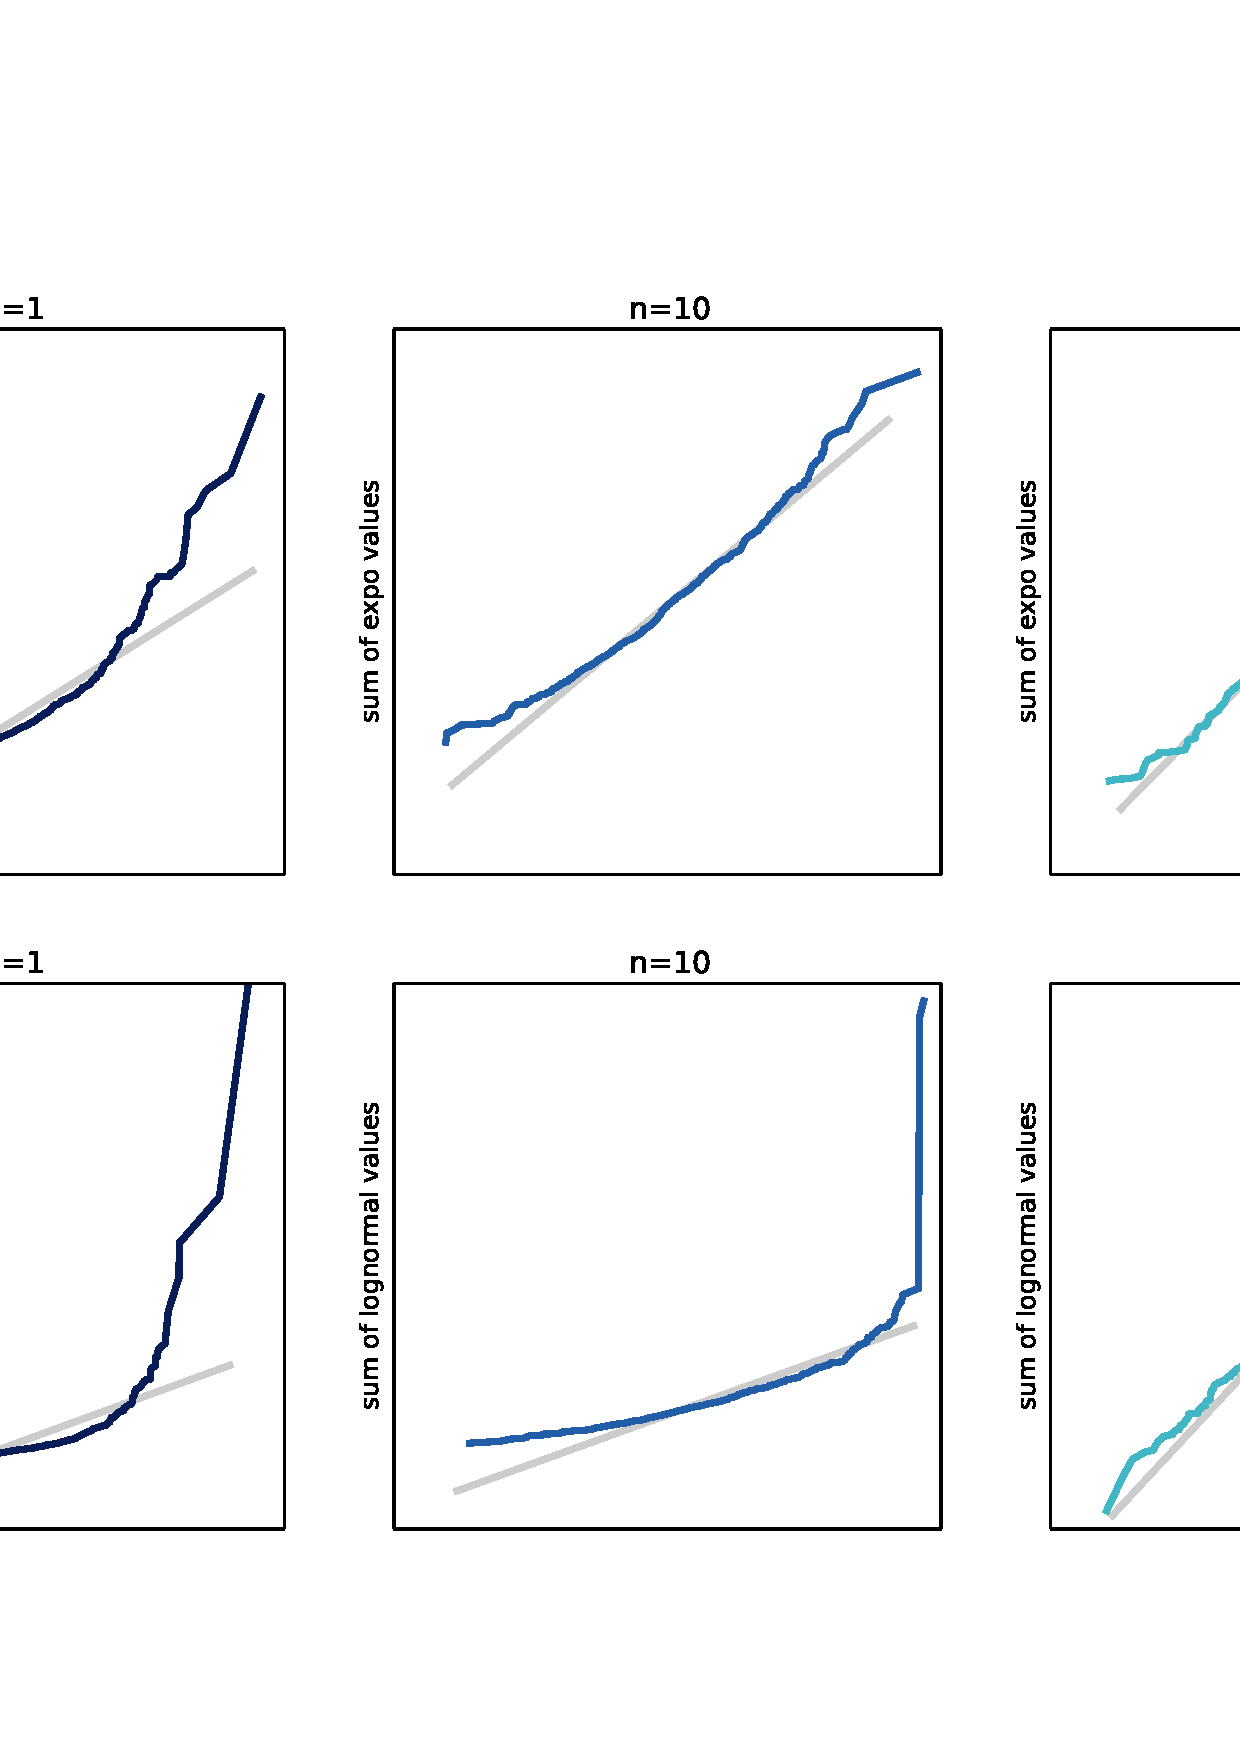
\includegraphics[height=3.5in]{figs/normal1.pdf}}
\caption{지수분포값의 합에 대한 분포(윗줄), 로그정규분포값의 합에 대한 분포(아랫줄).}
\label{normal1}
\end{figure}

그림~\ref{normal1} (위쪽 행)에 결과가 나와있다.
{\tt n=1}일 때, 합분포는 여전히 지수분포라서 정규확률그림은 직선이 아니다.
하지만, {\tt n=10}일 때, 합분포는 근사 정규분포가 되고,
{\tt n=100}일 때, 정규분포와 거의 구별되지 않는다.

그림~\ref{normal1} (아래 행)에 로그정규분포에 대한 비슷한 결과가 나와 있다.
로그정규분포는 일반적으로 지수분포보다 기울어짐이 더 심해서, 합분포는 수렴하는데 더 오래 걸린다. {\tt n=10}일 때, 정규확률그림은 거의 직선인 곳이 없다. 하지만, {\tt n=100}일 때, 근사적으로 정규분포다.
\index{로그정규 분포 (lognormal distribution)}
\index{분포 (distribution)!로그정규 (lognormal)}
\index{왜도 (skewness)}

\begin{figure}
% normal.py
\centerline{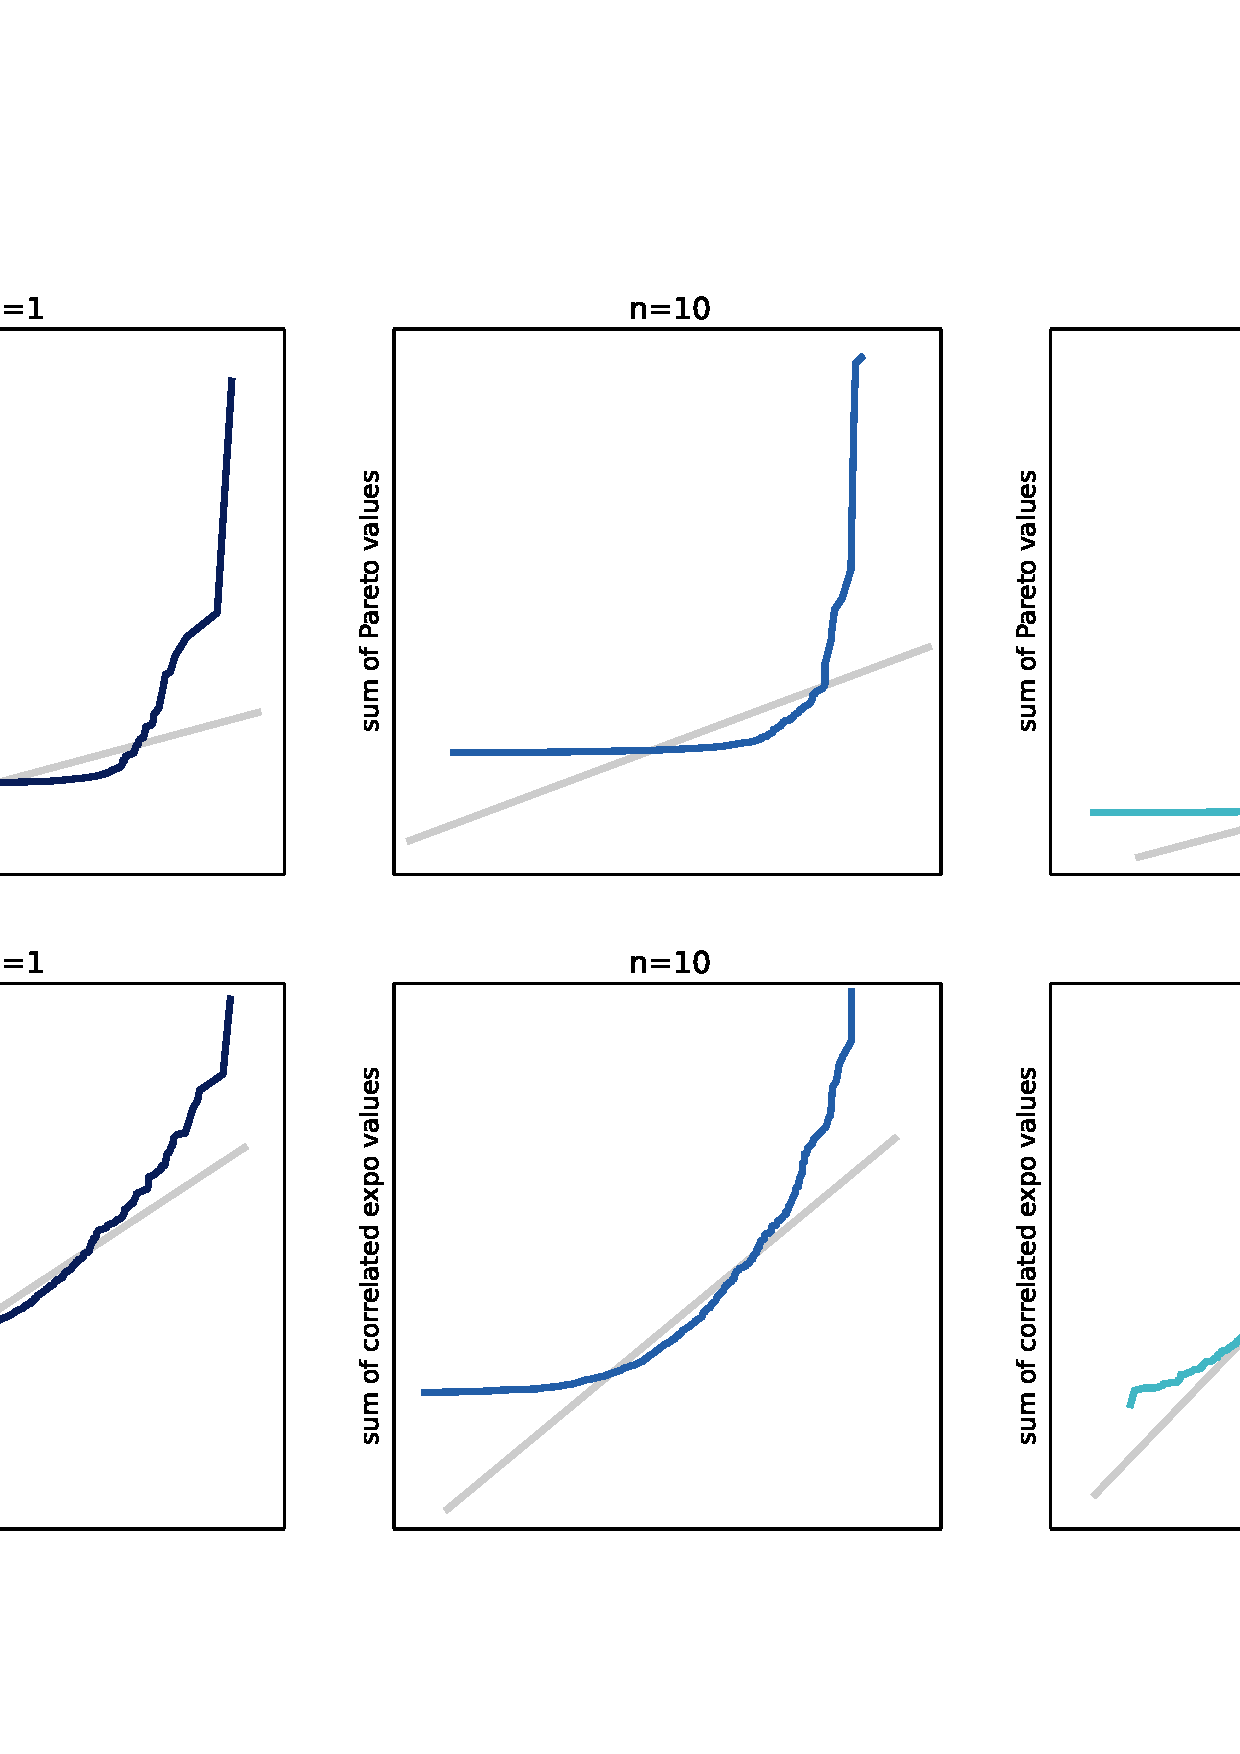
\includegraphics[height=3.5in]{figs/normal2.pdf}}
\caption{
파레토분포값의 합에 대한 분포(윗줄), 상관된 지수분포값의 합에 대한 분포(아랫줄).}
\label{normal2}
\end{figure}

파레토 분포는 로그정규분포보다 더 기울어짐이 심하다. 모수에 따라서, 많은 파레토 분포는 유한 평균과 분산을 갖지 못하다. 결과로, 중심극한정리가 적용되지 않는다. 그림~\ref{normal2} (상단 행)에 파레토 값들의 합 분포가 나와 있다. 심지어 {\tt n=100}일 때, 정규확률그림은 직선에서 거리가 멀다.
\index{파레토 분포 (Pareto distribution)}
\index{분포 (distribution)!파레토 (Pareto)}
\index{중심극한정리 (Central Limit Theorem)}
\index{CLT}
\index{정규확률그림 (normal probability plot)}

또한 CLT는 만약 값들이 상관된다면 적용되지 않는다고 언급했다. 이것을 검정하기 위해서, 지수분포에서 상관된 값들을 생성했다. 
상관된 값을 재생하는데 사용된 알고리즘은 (1) 상관된 정규분포 값을 발생시킨다. (2) 정규분포 CDF를 사용해서 값을 균등분포로 변환한다. (3) 역 지수분포 CDF를 사용해서 균등분포 값을 지수분포로 변환한다.

\index{역 CDF (inverse CDF)}
\index{CDF 역 (CDF, inverse)}
\index{상관 (correlation)}
\index{난수 (random number)}

{\tt GenerateCorrelated}는 계열상관 {\tt rho}를 갖는 {\tt n}개 정규분포 값 반복자를 반환한다.
\index{반복자 (iterator)}

\begin{verbatim}
def GenerateCorrelated(rho, n):
    x = random.gauss(0, 1)
    yield x

    sigma = math.sqrt(1 - rho**2)
    for _ in range(n-1):
        x = random.gauss(x*rho, sigma)
        yield x
\end{verbatim}

첫값은 표준정규분포 값이다. 각 후속값은 이전 값에 의존한다: 만약 이전 값이 {\tt x}, 다음값은 평균 {\tt x*rho}, 분산 {\tt 1-rho**2}이다. 
{\tt random.gauss}는 두번째 인자로 분산이 아닌 표준편차를 받는 것을 주목한다.
\index{표준편차 (standard deviation)}
\index{표준정규분포 (standard normal distribution)}

{\tt GenerateExpoCorrelated}는 결과 시퀀스를 인자로 받아 지수분포 값으로 변환한다.

\begin{verbatim}
def GenerateExpoCorrelated(rho, n):
    normal = list(GenerateCorrelated(rho, n))
    uniform = scipy.stats.norm.cdf(normal)
    expo = scipy.stats.expon.ppf(uniform)
    return expo
\end{verbatim}

{\tt normal}은 상관된 정규분포 값 리스트다.
{\tt uniform}은 0과 1사이 균등분포 값 시퀀스다.
{\tt expo}는 상관된 지수분포 값 시퀀스다.
{\tt ppf}는 ``퍼센트점 함수 (percent point function)''의 약어로 역CDF에 대한 또다른 이름이다.

\index{역CDF (inverse CDF)}
\index{CDF 역 (CDF, inverse)}
\index{퍼센트점 함수 (percent point function)}

그림~\ref{normal2} (하단 행)에 {\tt rho=0.9} 상관을 갖는 지수분포 값 합의 분포가 나와 있다. 상관된 경우 수렴속도가 느리다; 그럼에도 불구, {\tt n=100}일 때, 정규확률그림은 거의 직선이다. 그래서 값들이 상관되었을 때, CLT가 엄격하게 적용되지는 않지만, 적당한 상관은 실무에서 결코 문제가 되지 않는다.
\index{정규확률그림 (normal probability plot)}
\index{상관 (correlation)}

중심극한정리가 어떻게 동작하는지와 중심극한정리가 동작하지 않을 때 무슨일이 발생하는지 보여주기 위해서 이들 실험이 고안되었다. 이제 중심극한정리를 어떻게 사용하는지 살펴보자.


\section{CLT 적용하기}
\label{usingCLT}

왜 중심극한정리가 유용한지 살펴보기 위해서, ~\ref{testdiff}절에 예제로 돌아가자: 첫째아이와 첫째가 아닌 아이에 대한 평균 임신기간 외관효과 검정.
앞에서 살펴봤듯이, 외관 차이는 약 0.078주다.
\index{임신기간 (pregnancy length)}
\index{중심극한정리 (Central Limit Theorem)}
\index{CLT}

\begin{verbatim}
>>> live, firsts, others = first.MakeFrames()
>>> delta = firsts.prglngth.mean() - others.prglngth.mean()
0.078
\end{verbatim}

가설검정 로직을 기억하라: p-값을 계산하는데, 귀무가설 아래에서 관측 차이 확률이다; 만약 작다면, 관측 차이는 우연에 의한 것이 아닐 것으로 결론낸다.
\index{p-값 (p-value0}
\index{귀무가설 (null hypothesis)}
\index{가설검정 (hypothesis testing)}

이 예제애서, 귀무가설은 임신기간 분포가 첫째 아이와 첫째가 아닌 아이들에 대해서 같다. 그래서, 다음과 같이 평균 표집분포를 계산할 수 있다.
\index{표집분포 (sampling distribution)}

\begin{verbatim}
    dist1 = SamplingDistMean(live.prglngth, len(firsts))
    dist2 = SamplingDistMean(live.prglngth, len(others))
\end{verbatim}

두 표집분포는 동일 모집단에 기반하는데 모든 정상 출산을 합동(pool)한 것이다. {\tt SamplingDistMean}는 이 값 시퀀스와 표본크기를 인자로 받아 표집분포를 표현하는 Normal 객체를 반환한다.

\begin{verbatim}
def SamplingDistMean(data, n):
    mean, var = data.mean(), data.var()
    dist = Normal(mean, var)
    return dist.Sum(n) / n
\end{verbatim}

{\tt mean}와 {\tt var}는 {\tt data} 평균과 분산이다.
정규분포 {\tt dist}로 데이터 분포를 근사한다.

이 예제애서 데이터는 정규분포되어 있지 않다. 그래서 이러한 근사가 그다지 좋지 않다. 하지만 그리고 나서 {\tt dist.Sum(n) / n}을 계산하는데 {\tt n}개 값 평균의 표집분포다. 데이터가 정규분포되어 있지 않지만, 평균 표집분포는 중심극한정리에 의해서 정규분포된다.
\index{중심극한정리 (Central Limit Theorem)}
\index{CLT}

다음, 평균에 차이 표집분포를 계산한다.
{\tt Normal} 클래스는 방정식 2를 사용해서 뺄셈을 어떻게 수행하는지 알고 있다.
\index{Normal}

\begin{verbatim}
    def __sub__(self, other):
        return Normal(self.mu - other.mu,
                      self.sigma2 + other.sigma2)
\end{verbatim}

그래서, 다음과 같이 차이 표집분포를 계산할 수 있다.

\begin{verbatim}
>>> dist = dist1 - dist2
N(0, 0.0032)
\end{verbatim}

평균은 0 인데, 일리가 있다. 왜냐하면 평균적으로 동일 분포에서 추출된 두 표본은 같은 평균을 갖을 것으로 예상하기 때문이다. 표집분포 분산은 0.0032가 된다.
\index{표집분포 (sampling distribution)}

{\tt Normal} 클래스는 {\tt Prob}메쏘드를 제공하는데 정규분포 CDF를 평가한다. {\tt Prob}를 사용해서 귀무가설 아래에서 차이 확률을 {\tt delta} 만큼 계산할 수 있다.
\index{귀무가설 (null hypothesis)}

\begin{verbatim}
>>> 1 - dist.Prob(delta)
0.084
\end{verbatim}

의미하는 바는 단측검정에 대한 p-값이 0.084다. 양측검정에 대해서 또한 다음과 같이 계산한다.
\index{p-값 (p-value)}
\index{단측검정 (one-sided test)}
\index{양측검정 (two-sided test)}

\begin{verbatim}
>>> dist.Prob(-delta)
0.084
\end{verbatim}

정규분포는 대칭이기 때문에 동일하다. 꼬리 합은 0.168로, ~\ref{testdiff}절 추정값과 일치한다; 값이 0.17이였다.
\index{대칭(symmetric)}



\section{상관검정 (Correlation test)}

~\ref{corrtest}절에서 출생 체중과 산모 연령 사이 상관을 계산하는데 순열검정(permutation test)을 사용했고, p-값이 0.001보다 작아 통계적으로 유의적이라는 것을 발견했다.
\index{p-값 (p-value)}
\index{출생체중 (birth weight)}
\index{체중 (weight)!출생 (birth)}
\index{순열 (permutation)}
  \index{유의성 (significant)} 
  \index{통계적 유의성 (statistically significant)}

이제 해석적으로 같은 것을 수행할 수 있다.
메쏘드는 다음 수학적 결과에 기반한다: 정규분포를 따르고 상관되지 않는 두변수가 주어지고, 만약 $n$개 크기 표본을 생성하고, 피어슨 상관 $r$을 계산하고 나서, 변환된 상관을 계산하면, 
%
\[ t = r \sqrt{\frac{n-2}{1-r^2}} \]
%
$t$분포는 모수 $n-2$을 갖는 스튜던트 t-분포다.
t-분포는 해석적 분포다; CDF는 감마 함수를 사용해서 효율적으로 계산될 수 있다.
\index{피어슨 상관계수 (Pearson coefficient of correlation)}
\index{상관 (correlation)}

이 결과를 사용해서 귀무가설 아래에서 상관 표집분포를 계산할 수 있다; 즉, 만약 상관되지 않은 정규분포 값 시퀀스를 생성한다면, 두 시퀀스 상관 분포는 무엇일까요? {\tt StudentCdf}가 표본크기 {\tt n}을 인자로 받아 상관 표집분포를 반환한다.
\index{귀무가설 (null hypothesis)}
\index{표집분포 (sampling distribution)}

\begin{verbatim}
def StudentCdf(n):
    ts = np.linspace(-3, 3, 101)
    ps = scipy.stats.t.cdf(ts, df=n-2)
    rs = ts / np.sqrt(n - 2 + ts**2)
    return thinkstats2.Cdf(rs, ps)
\end{verbatim}

{\tt ts}는 $t$에 대한 값 넘파이(NumPy) 배열, 변환 상관이다.
{\tt ps}는 대응되는 확률을 담고 있는데, SciPy로 구현된 스튜던트 t-분포 CDF를 사용해서 계산된다. t-분포 모수, {\tt df}는 ``자유도 (degrees of freedom)''의 두문자(acronym)다. 이 용어를 설명하지는 않지만, 웹사이트에서 자세한 내용 참조한다. \url{http://en.wikipedia.org/wiki/Degrees_of_freedom_(statistics)}.
\index{넘파이 (NumPy)}
\index{SciPy}
\index{스튜던트 t-분포 (Student's t-distribution)}
\index{분포 (distribution)!스튜던트 t (Student's t)}
\index{자유도 (degrees of freedom)}

\begin{figure}
% normal.py
\centerline{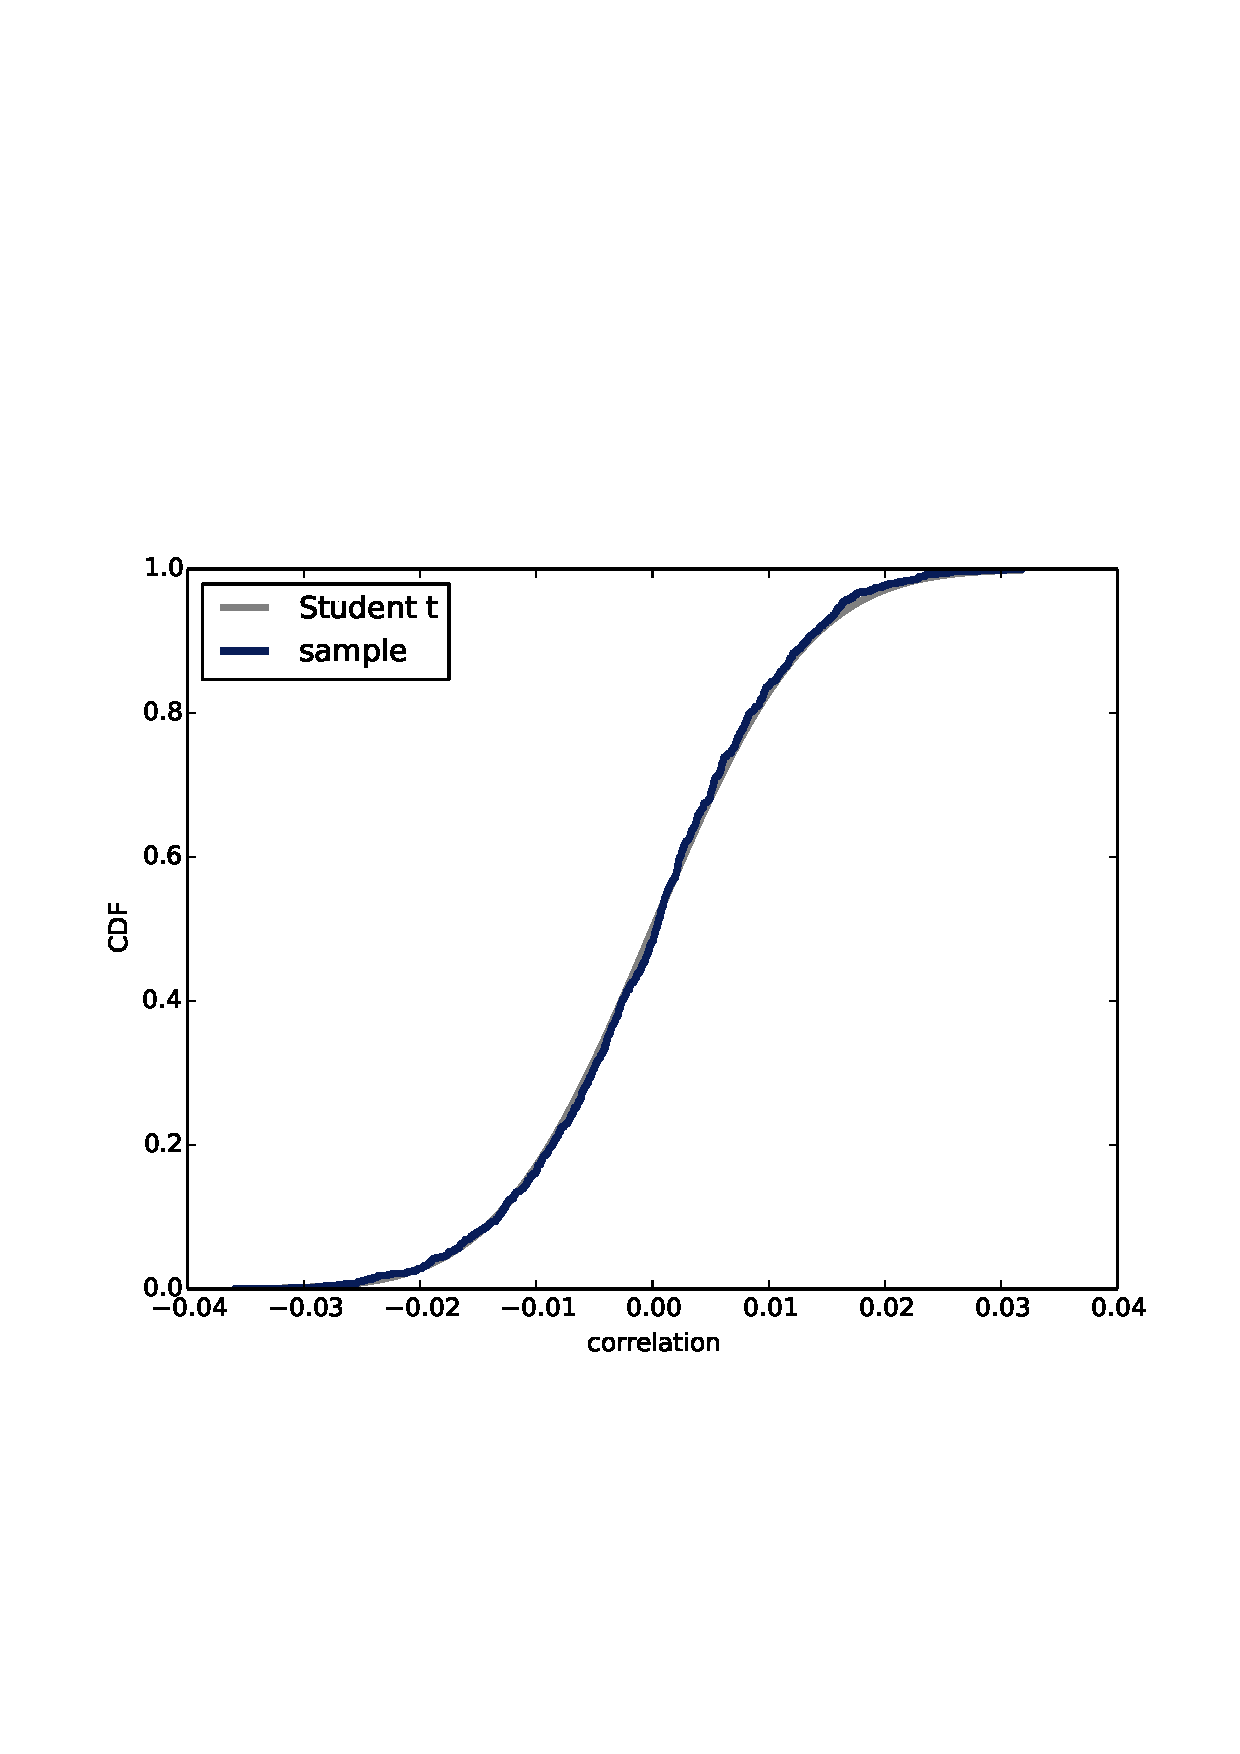
\includegraphics[height=2.5in]{figs/normal4.pdf}}
\caption{상관되지 않은 정규변수에 대한 상관계수에 대한 표집분포.}
\label{normal4}
\end{figure}

{\tt ts}로부터 상관계수 {\tt rs}를 얻기 위해서, 역변환을 적용한다.
%
\[ r = t / \sqrt{n - 2 + t^2} \]
%
결과는 귀무가설 아래에서 $r$의 표집분포가 된다.
그림~\ref{normal4}에 재표본추출로 ~\ref{corrtest}절에서 생성한 분포를 따라 이 분포를 함께 보여준다.
두 분포가 거의 동일(identical)하다. 실제 분포가 정규분포는 아니지만, 피어슨 상관계수는 표본 평균과 분산에 기반한다. 중심극한정리에 의해서, 설사 데이터는 그렇지 않지만, 적률기반 통계량은 정규분포한다.

\index{중심극한정리 (Central Limit Theorem)}
\index{CLT}
\index{귀무가설 (null hypothesis)}
\index{재표본추출 (resampling)}

그림 ~\ref{normal4}로부터, 만약 변수가 실제로 상관되지 않는다면, 관측 상관 0.07은 일어날 것 같지 않다는 것을 볼 수 있다. 해석 분포를 사용해서, 얼마나 그럴것 같지 않은지를 계산할 수 있다.
\index{해석 분포 (analytic distribution)}

\begin{verbatim}
    t = r * math.sqrt((n-2) / (1-r))
    p_value = 1 - scipy.stats.t.cdf(t, df=n-2)
\end{verbatim}

{\tt r=0.07}에 상응하는 {\tt t} 값을 계산한다. 그리고 나서 {\tt t}에 t-분포를 평가한다. 결과는 {\tt 6.4e-12}가 나온다.
이 예제는 해석적 방법의 장점을 시연한다: 매우 작은 p-값을 계산할 수 있다. 하지만, 실무에서 보통 문제가 되는 않는다.
\index{SciPy}
\index{p-값 (p-value)}


\section{카이제곱 검정 (Chi-squared test)}

~\ref{casino2}절에서 카이제곱 통계량을 사용해서 주사위가 비뚤었는지 검정했다. 카이제곱 통계량은 표(table)에 기대값과 정규화된 총 편차를 측정한다:
%
\[ \goodchi^2 = \sum_i \frac{(O_i - E_i)^2}{E_i} \]
%
카이제곱 통계량이 널리 사용되는 이유는 귀무가설 아래에서 표집분포가 해석적(analytic)이기 때문이다; 놀라운 우연의 일치\footnote{정말.(Not really.)}로, 카이제곱 분포로 불린다.
t-분포처럼 카이제곱 CDF는 감마 함수를 사용해서 효율적으로 계산될 수 있다.
\index{편차 (deviation)}
\index{귀무가설 (null hypothesis)}
\index{표집분포 (sampling distribution)}
\index{카이제곱 검정 (chi-squared test)}
\index{카이제곱 분포 (chi-squared distribution)}
\index{분포 (distribution)!카이제곱 (chi-squared)}

\begin{figure}
% normal.py
\centerline{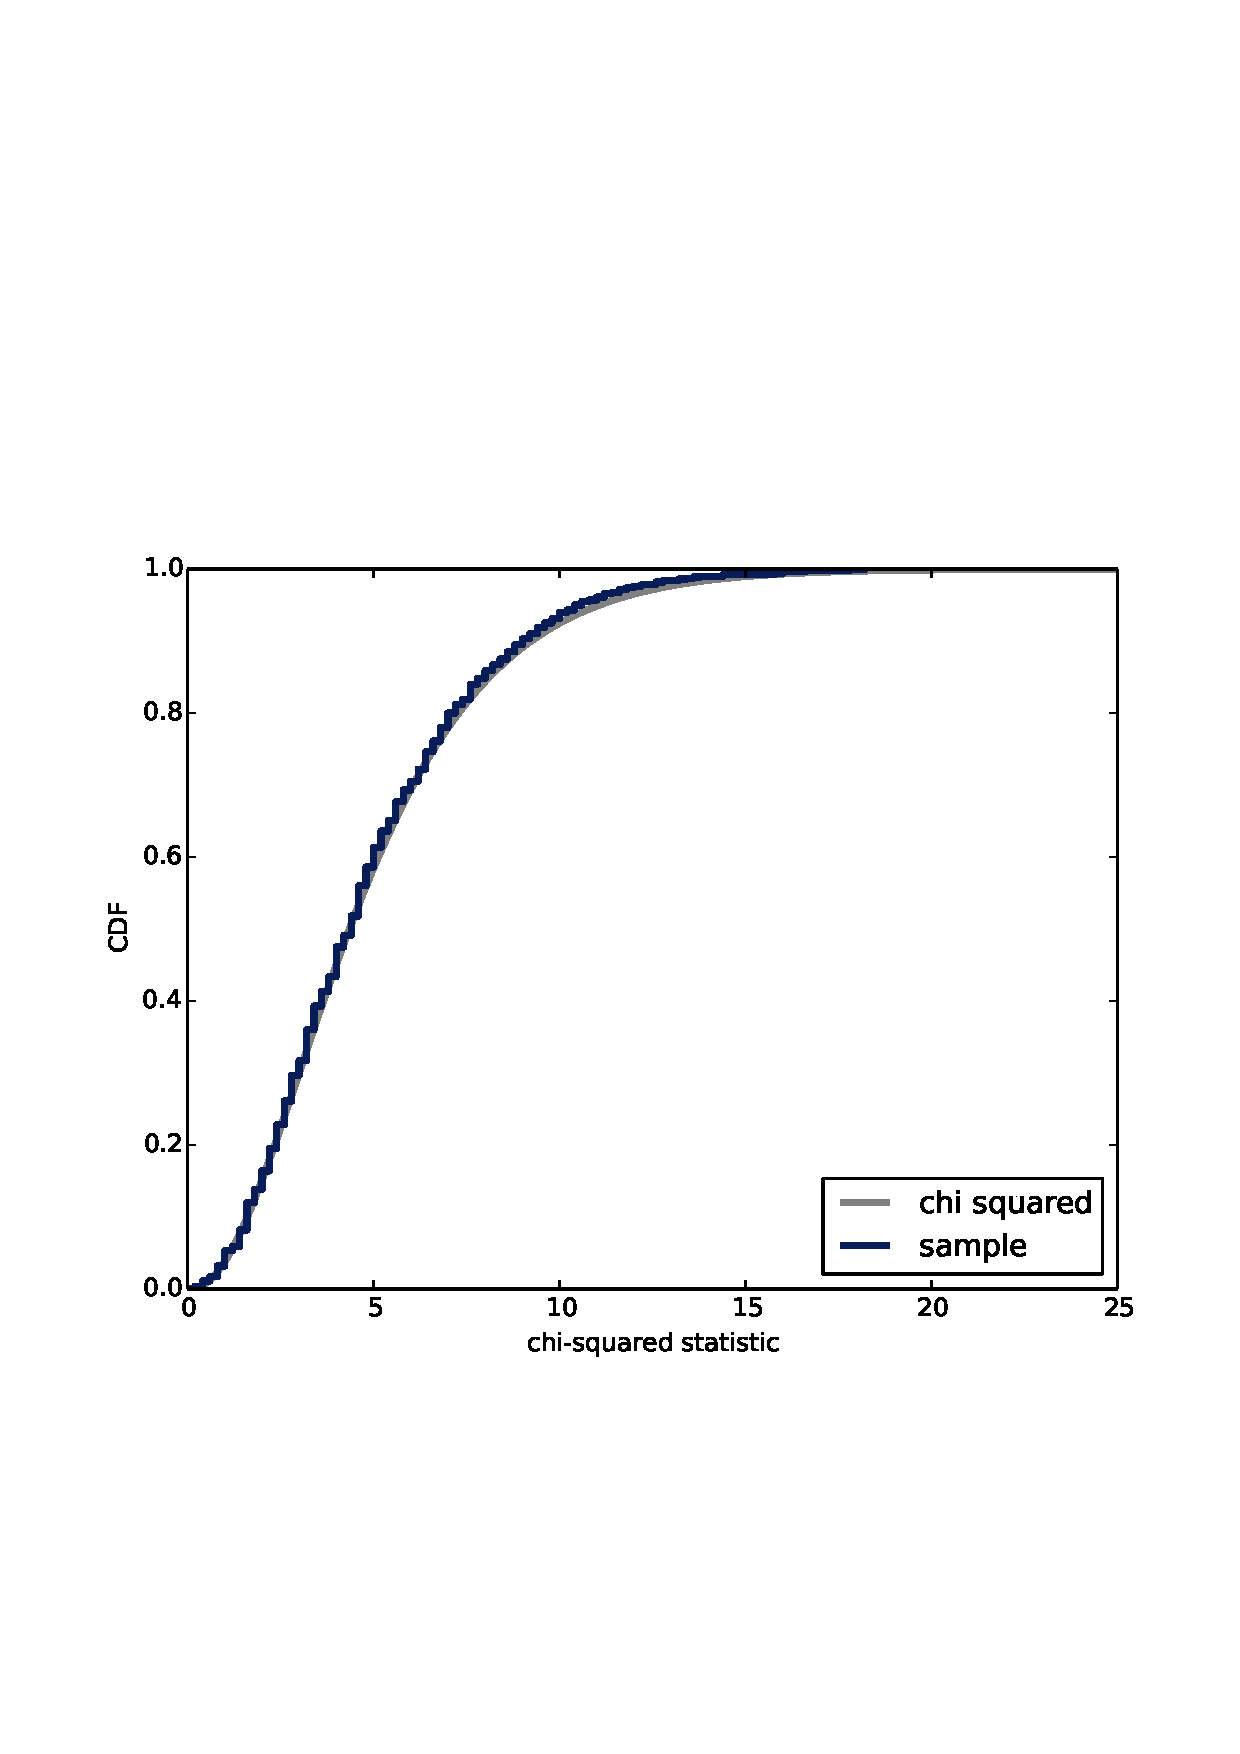
\includegraphics[height=2.5in]{figs/normal5.pdf}}
\caption{치우침없는 6각 주사위에 대한 카이제곱 통계량에 대한 표집분포.}
\label{normal5}
\end{figure}

SciPy는 카이제곱 분포 기능을 제공한다. 이것을 사용해서 카이제곱 통계량 표집분포를 계산한다.
\index{SciPy}

\begin{verbatim}
def ChiSquaredCdf(n):
    xs = np.linspace(0, 25, 101)
    ps = scipy.stats.chi2.cdf(xs, df=n-1)
    return thinkstats2.Cdf(xs, ps)
\end{verbatim}

그림~\ref{normal5}에 재표본추출로 얻은 분포와 함께 해석적 결과가 함께 나와 있다. 둘다 모두 매우 비슷한데, 특히 꼬리부분에 그렇다. 꼬리부분은 통상 가장 관심을 두는 부분이다.
\index{재표본추출 (resampling)}
\index{꼬리 (tail)}

이분포를 사용해서 관측 검정 통계량, {\tt chi2}의 p-값을 계산할 수 있다:
\index{검정 통계량 (test statistic)}
\index{p-값 (p-value)}

\begin{verbatim}
    p_value = 1 - scipy.stats.chi2.cdf(chi2, df=n-1)
\end{verbatim}

결과는 0.041로 ~\ref{casino2}절 결과와 일치한다.

카이제곱 분포 모수는 다시 ``자유도(degrees of freedom)''가 된다.
이 경우 맞는 모수는 {\tt n-1}ㅇ 되는데, 여기서 {\tt n}은 표(table) 크기로 6이다.
이 모수를 선택한 것이 다소 까다로울 수 있다; 정직하게 해석결과와 재표본추출 결과를 비교하기 위해서, 그림~\ref{normal5}같은 것을 생성할 때가지 저자는 그것이 맞는지 확신할 수 없었다.
\index{자유도 (degrees of freedom)}


\section{토의 (Discussion)}

이책은 재표본추출과 순열 같은 수치해석적 방법(computational method)에 집중했다. 이 방법이 해석적인 방법에 대해서 몇가지 장점이 있다.

\index{재표본추출 (resampling0}
\index{순열 (permutation)}
\index{수치해석적 방법 (computational methods)}

\begin{itemize}

\item 수치해석적 방법이 설명하고 이해하기 더 쉽다. 예를 들어, 기초 통계에서 가장 어려운 주제가 가설검정이다. 많은 학생이 p-값이 무엇인지 정말 이해하지 못한다. ~\ref{testing}장에서 제시한 접근법---귀무가설을 모의시험하고 검정 통계량을 계산하는 것---이 근본개념을 좀더 명확하게 한다고 믿는다.
\index{p-값 (p-value)}
\index{귀무가설 (null hypothesis)}

\item 수치해석적 방법이 강건하고 다목적이다. 해석적 방법은 실무에서 지지할 수 없는 가정에 종종 기반한다. 수치해석적 방법은 더 적은 가정을 요구하고 좀더 쉽게 확장과 개조를 할 수 있다.
\index{강건성 (robust)}

\item 수치해석적 방법은 디버그(debuggable)할 수 있다. 해석적 방법은 종종 블랙박스다: 숫자를 집어 넣으면 결과가 튀어나온다. 하지만 미묘한 실수를 하기 쉽고, 결과가 맞는지 확신하기 어렵다. 그리고 만약 문제가 없다면 문제를 찾기가 어렵다. 수치해석적 방법은 점증 개발 및 테스트(incremental development and testing)를 할 수 있게 해서 결과에 신뢰감을 함양한다.
\index{디버깅 (debugging)}

\end{itemize}

하지만, 한가지 단점이 있다: 수치해석적 방법은 느릴 수 있다.
장점과 단점을 고려해서, 다음 과정(process)를 추천한다.

\begin{enumerate}

\item 탐색과정에서 수치해석적 방법을 사용하라. 만약 만족스러운 답을 찾고 실행시간이 수용가능하면, 멈출 수 있다.
\index{탐색 (exploration)}

\item 만약 실행시간을 받아들일 수 없다면, 최적화할 기회를 찾아봐라. 해석적 방법을 사용하는 것은 몇가지 최적화 방법중 하나다.

\item 만약 수치해석적 방법을 해석적 방법으로 바꾸는 것이 적절하다면, 수치해석적 방법을 비교 기반으로 사용하라. 왜냐하면 수치해석적 결과와 해석적 결과 사이에 상호 타당성 검증기능을 제공하기 때문이다.
\index{모형 (model)}

\end{enumerate}

저자가 해결하려고 노력한 방대한 문제에 대해서, 1단계를 지나갈 필요는 없다.


\section{연습 문제}

이 연습문제에 대한 해답은 \verb"chap14soln.py" 파일에 나와 있다.

\begin{exercise}
\label{log_clt}

\ref{lognormal}~절에서, 성인 체중분포는 근사적으로 로그정규분포임을 알아냈다.
한가지 가능한 설명은 매년 성인이 느는 체중은 현재 체중에 비례한다는 것이다.
이런 경우, 성인 체중은 많은 숫자의 복잡한 요인의 곱이 된다:

%
\[ w = w_0 f_1 f_2 ... f_n  \]
%

여기서, $w$는 성인체중, $w_0$는 출생체중,
$f_i$는 $i$ 년도에 대한 체중 증가 요인이다.

\index{출생체중}
\index{체중!출생}
\index{로그정규 분포}
\index{분포!로그정규}
\index{성인체중}

곱에 대해 로그를 취하면, 요인에 로그를 취한 합으로 바뀐다:
%
\[ \log w = \log w_0 + \log f_1 + \log f_2 + ... + \log f_n \]
%

그래서, 중심극한정리에 의해서, 
$\log w$의 분포는 근사적으로 큰 $n$에 대해 근사적으로 정규분포가 된다.
이는 $w$의 분포가 로그정규분포라는 것을 함의를 갖는다.
\index{중심극한정리}
\index{CLT}

이런 현상을 모형화하는데, $f$에 대한 일리있어 보이는 분포를 고르고 나서,
출생체중 분포로 부터 난수를 고르고, $f$ 분포로부터 요인 시퀀스를 고르고,
곱을 계산함으로써 성인체중 표본을 생성한다.
로그정규 분포로 수렴하는데 $n$ 값이 얼마나 필요할까?

\index{모형}

\index{로그}
\index{곱}

\end{exercise}



\begin{exercise}

\ref{usingCLT}~절에서, 중심극한정리를 사용해서 
동일 모집단에서 양쪽 표본이 추출되었다는 귀무가설 아래,
평균간에 차이, $\delta$, 표집분포를 알아냈다.
\index{귀무가설}
\index{표집분포}

이 분포를 사용해서 추정값 표준오차와 신뢰구간도 알아낼 수 있다.
하지만, 이 방식은 근사적으로 맞다.
좀더 정확성을 기하기 위해서, 표본이 다른 모집단에서 추출되었다는
대립가설 아래 $\delta$ 표집분포를 계산해야 된다.
\index{표준오차}
\index{표준편차}
\index{신뢰구간}

이 분포를 계산하고, 이를 사용해서 평균 사이 차이에 대한 
표준오차와 90\% 신뢰구간을 계산하시오.
\end{exercise}


\begin{exercise}
최신 논문\footnote{``Evidence for the persistent effects of an
  intervention to mitigate gender-sterotypical task allocation within
  student engineering teams,'' Proceedings of the IEEE Frontiers in Education
Conference, 2014.}에서, 스타인과 동료들은 
학생공학팀 안에서 성별 고정관념에 따른 작업 배정을 완화하려는 의도로 개입 효과를 조사했다.

개입 전과 후에 대해서, 학생들이 7점 척도로 학급 프로젝트 각 측면에 대한 기여도를 
평가하는 설문에 응답했다.

개입 전에는, 남자 학생이 여자 학생보다 프로젝트의 프로그래밍 측면에 대해서
더 높은 점수를 보고했다; 평균적으로 남자가 0.28 표준오차를 갖는 3.57
점수를 보고했다. 여자는 평균적으로 0.32 표준오차를 갖는 1.91을 보고했다.
\index{표준오차}

성별 격차(평균에 있어 차이)에 대한 표집분포를 계산하고,
통계적으로 유의적인지 검정하라.
추정한 평균에 대한 표준오차만 주어졌기 때문에,
표집분포를 식별하는데 표본크기를 알 필요는 없다.
  \index{유의적인} \index{통계적으로 유의적인}
\index{표집분포}

개입후에, 성별격차가 더 적어졌다:
남자에 대한 평균점수는 3.44 (표준오차 0.16); 여자에 대한 평균점수 3.18 (표준오차 0.16).
다시, 성별격차에 대한 표집분포를 계산하고 검정하라.
\index{성별격차}

마지막으로 성별격차에 변화를 추정하라; 이 변화에 대한 표집분포는 무엇이고,
통계적으로 유의적인가?
  \index{유의적인} \index{통계적으로 유의적인}
\end{exercise}
